\section{Termination Analysis via Interpolation-based Transition Invariant Generation}

We propose a new approach for proving termination that leverages safety verification to generate a well-founded transition invariant
candidate via interpolation.
At each iteration, our procedure constructs a trace from the initial states to a sink state.
A well-founded transition invariant is then constructed based on the overapproximation of the terminating trace.
If the invariant is valid for all reachable states, termination is concluded. 
The interpolation-based approach enables efficient property-directed transition invariant generation, as it is constructed with respect to the termination condition.

\subsection{Interpolation-based Generation of Well-Founded Transition Invariants}

The core of our approach is the procedure for automated, interpolation-based generation of 
well-founded transition invariants: \trInvSynthesis. 
Given a transition system and a terminating trace, the procedure 
constructs a disjunctively well-founded approximation of the transition trace. 
If the resulting formula constitutes a transition invariant over all reachable states, 
it witnesses termination.

The Procedure consists of five major steps:
% (1) computing $T^n$, the formula encoding states that terminate within $n$ transitions.
% $T^n$ is used to construct the interpolant. It guarantees that no states other then $Sink$ are reachable in $n$ transitions; 
(1) computing $NT^n$, the formula encoding states that do not necessarily terminate within $n$ transitions.
$NT^n$ is used to construct the interpolant. The negation of $NT^n$ defines the states that necessarily reach $Sink$ 
in at most $n$ transitions; 
(2) constructing an over-approximation of the terminating trace via interpolation. 
The usage of sink states allows the interpolant to capture the reason for termination; 
(3) converting the interpolant into an underapproximating DNF formula.
This allows to efficiently synthesise ranking functions for separate disjuncts; 
(4) filtering disjuncts to retain only those encoding well-founded relations, constructing a candidate transition invariant.
Only well-founded relations are saved, as transition invariant needs to be disjunctively well-founded to witness termination; and 
(5) computing the formula encoding states for which candidate formula is a valid transition invariant.
Transition invariant needs to be valid only over the reachable states to conclude termination.
Therefore, if all reachable states satisfy this formula - TS is terminating.
The overall flow of the procedure is illustrated in the Figure~\ref{fig:TrInvGen}.

\begin{figure}[t]
    \centering
    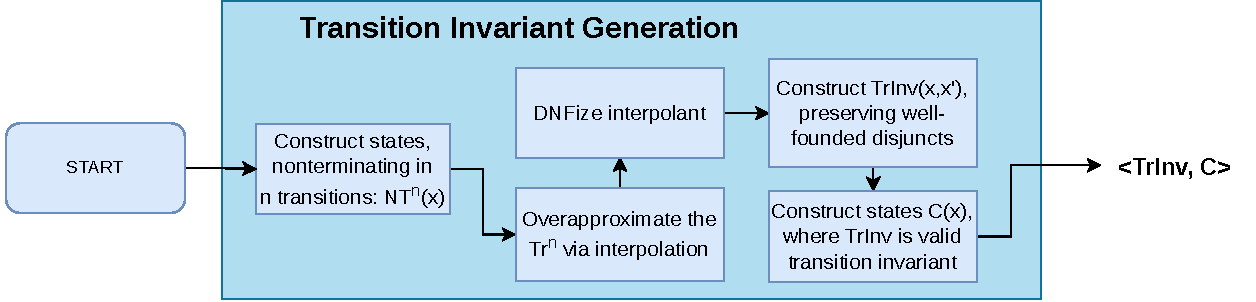
\includegraphics[width=\linewidth]{Figures/TrInv.pdf}
    \caption{Execution Flow of Interpolation-based Transition Invariant Generation}
    \label{fig:TrInvGen}
\end{figure}


\begin{algorithm}[t!]
	\SetInd{0.5em}{0.5em}
    \DontPrintSemicolon
    \small
    \newcommand{\Continue}{\textbf{continue}}
    \caption{$\trInvSynthesis(P, Tr^n, TInv)$.}
    \label{Alg:SNA_TrInv}
    \SetKwInOut{Input}{Input}
    \SetKwInOut{Output}{Output}
    \Input{Safety problem $P = \tuple{Init, Tr, Sink, X}$, transition trace $Tr^n(X^{(0)}, X^{(1)}, \dots, X^{(n)})$, candidate transition invariant $TInv(X,X')$}
    \Output{Updated transition invariant $TInv(X,X')$ and formula $C(X)$ encoding states covered by
    transition invariant}
    $NT^n(X^{(0)}) \gets  QE(\exists X^{(1)}, \dots, X^{(n)}.$ $Tr^{n}(X^{(0)}, X^{(1)}, \dots, X^{(n)}) \land \lnot Sink(X^{(n)}))$ \label{SNA_TrInv:T} \\
    % $T^n(X^{(0)}) \gets \lnot QE(\exists X^{(1)}, \dots, X^{(n)}.$ $Tr^{n}(X^{(0)}, X^{(1)}, \dots, X^{(n)}) \land \lnot Sink(X^{(n)}))$ \label{SNA_TrInv:T} \\
    % $itp(X,X') \gets Itp(Tr^{n}(X, \dots, X'), T^n(X) \land \lnot Sink(X'))$\label{SNA_TrInv:Itp}\\
    $itp(X,X') \gets Itp(Tr^{n}(X, \dots, X'), \lnot NT^n(X) \land \lnot Sink(X'))$\label{SNA_TrInv:Itp}\\
    $Cs(X,X') \gets toDNF(itp)$ \label{SNA_TrInv:toDNF}\\
    $TInv \gets TInv \lor \bigvee_i \{d_i \in Cs| \text{$\exists$ ranking function $f(X)$} \}$\label{SNA_TrInv:TINV} \\
    $C(X) \gets \lnot QE(\exists X',X''.$ $\bigl(Id(X,X') \lor TInv(X,X')\bigr)  \land Tr(X',X'') 
        \land \lnot TInv(X,X''))$ \label{SNA_TrInv:NC} \\
    \Return $\tuple{TInv, C}$
\end{algorithm}

Algorithm~\ref{Alg:SNA_TrInv} takes as an input a safety problem $P = \tuple{Init, Tr, Sink, X}$,
a transition trace $Tr^n(X^{(0)}, X^{(1)}, \dots, X^{(n)})$, and a transition invariant formula $TInv(X,X')$. 
It returns a tuple of formulas $\tuple{TInv, C}$, where $TInv(X,X')$ is a disjunctively well-founded transition invariant 
candidate, and $C(X)$ is a formula encoding the states for which $TInv$ is a valid transition invariant. 
It proceeds in the following steps:
% Define from the negation, not the itself

\textbf{Step 1}: \textit{Computing $NT^n$ (line~\ref{SNA_TrInv:T}).} 
$NT^n(X)$ encodes all states that do not necessarily terminate in $n$ 
transitions, is defined by the following property:
% $NT^n(X)$ encodes all states guaranteed to reach a sink state within $n$ 
% transitions, is defined by the following property:

$$\exists X^{(0)}, \dots, X^{(n)}. Tr^{n}(X^{(0)}, \dots, X^{(n)}) \land \lnot Sink(X^{(n)})$$

$NT^n$ is constructed with quantifier elimination, eliminating all variables from the formula except for $X^{(0)}$.
Construction of $NT^{(n)}$ enables the overapproximation of the trace. 

\begin{example}\label{Ex:Tn}
    % Consider $TS = \tuple{Init, Tr, X}$ with $Init \triangleq  x > 0$, $Tr(X,X') \triangleq  ((x' = x - 1 \lor x' = x - 2) \land x > 0) \lor (x < -10 \land x' = x - 1)$, $X \triangleq  \{x\}$.
    % For $n = 2$ quantifier elimination would yield $T^2(X) = x \leq 2$.
    % States with $x \in \{3,4\}$ can reach $Sink$ in two transitions but are 
    % not guaranteed to do so, so they are not included in $T^2$.
    % States with $x \in \{1,2\}$ terminate in 1 or 2 transitions.
    Consider $TS = \tuple{Init, Tr, X}$ with $Init \triangleq  x > 0$, $Tr(X,X') \triangleq  ((x' = x - 1 \lor x' = x - 2) \land x > 0) \lor (x < -10 \land x' = x - 1)$, $X \triangleq  \{x\}$.
    In this TS, sink states can be encoded as $Sink(X) \triangleq x \leq 0 \land x \geq -10$.
    For $n = 2$ quantifier elimination would yield $NT^2(X) = x > 2$.
    States with $x \in \{3,4\}$ can reach $Sink$ in two transitions, but not necessarily.
    Therefore these states are included in $NT^2$.
\end{example}

\textbf{Step 2}: \textit{Interpolation (line ~\ref{SNA_TrInv:Itp}).}
The following formula is unsatisfiable by construction, since any state in 
$\lnot NT^n$ must reach $Sink$ within $n$ steps:

$$\lnot NT^{n}(X^{(0)}) \land Tr^{n}(X^{(0)}, \dots, X^{(n)}) \land \lnot Sink(X^{(n)})$$

This allows to compute the \textbf{Craig interpolant}, which over-approximates the trace $Tr^{n}$.
Crucially, the usage of the sink states for interpolant construction allows the interpolant to capture the reason \emph{why} 
the particular trace is terminating.



\textbf{Step 3}: \textit{DNF underapproximation (line ~\ref{SNA_TrInv:toDNF}).}
For a transition invariant to witness termination, it must be 
disjunctively well-founded, meaning every disjunct must encode a 
well-founded relation. Converting the interpolant to a full DNF 
would make each disjunct a conjunction, simplifying the 
well-foundedness check, but full DNF conversion can cause an 
exponential blowup in formula size. Moreover, even a complete DNF 
is not guaranteed to yield a transition invariant or to witness 
termination.

Instead, our algorithm follows a lazy approach: it constructs an 
under-approximating DNF formula on demand. 
Concretely, algorithm constructs disjuncts as follows:
(1) SMT solver prodices a model that satisfies $itp$, (2) 
Using produced model, the satisfied literals are extracted from the SMT formula and conjoined,
(3) This conjunction is one of the dinsjuncts in the constructed DNF. It is blocked from the itp, 
and the dnfization proceeds (until reaching certain limit).
The result is a formula:
$$Cs(X,X') \triangleq \bigvee_{i=0}^m d_i$$
where each $d_i$ is a conjunction, and $Cs(X,X') \rightarrow itp(x,x')$.
This approach significantly reduces formula size and speeds up both DNFization and 
subsequent well-foundedness check, while preserving correctness: 
in the worst case, $Cs$ fails to be a transition invariant over all 
reachable states, but this is equally possible even with a complete DNF conversion.
% Empirically, bounding the number of disjuncts produces more 
% compact and efficiently verifiable termination proofs.
% Our algorithm produces a model satisfying the SMT formula.
% Using produced model, it extracts the satisfied literals from the SMT formula, and constructs a conjunction of these literals.
% This conjunction is one of the dinsjuncts in the constructed DNF. This conjunction is blocked in the original formula, and the process proceeds.
% It allows to significantly reduce the size of the resulting formula and speed up the DNF conversion, while preserving correctness: 
% in the worst case, the resulting formula is not a transition invariant (which can happen even if the complete DNF is produced).
% Empirically, we observed that limiting the number of disjuncts results in more size-efficient and quick termination proofs.
% The execution of the procedure returns a formula:

% The number of disjuncts is bounded by a constant (a tunable parameter depending on the available size of RAM), since DNF 
% conversion can cause an exponential blowup in formula size.  Move to implementation & evaluation
% Bring citation 3 to background section

\textbf{Step 4}: \textit{Filtering Well-Founded Disjuncts (line ~\ref{SNA_TrInv:TINV}).}
For each disjunct $d(X,X') \in Cands(X,X')$ algorithm checks if $d(X,X')$ encodes a well-founded relation.
Our technique uses automated linear ranking function synthesis~\cite{DBLP:conf/vmcai/PodelskiR04} for checking the existence of a ranking function.
The disjuncts for which a ranking function exists are preserved, and the rest are discarded.
The resulting formula is disjoined with the input candidate transition invariant $TInv$.

\textbf{Step 5}: \textit{Synthesis of the states for which transition invariant is valid (line ~\ref{SNA_TrInv:NC}).}
If $TrInv$ is a transition invariant over all reachable states, then TS terminates, since every disjunct corresponds to well-founded relation.
To verify this, procedure computes the formula $C(X)$ encoding the states over which $TrInv$ is a valid transition invariant. 
% Split this thing into 2 properties
% Make it consistent with the code
\begin{definition}[Coverage formula]
    Consider a transition system $TS = \tuple{Init, Tr, X}$ and a formula $TrInv(X,X')$. 
    We say that $C(X)$ is a coverage formula, if the following properties hold $\forall X, X',X''$:
    \begin{align*}
     C(X) \land Tr(X,X') \rightarrow& TrInv(X,X') \\
     C(X) \land TrInv(X,X') \land Tr(X',X'') \rightarrow& TrInv(X,X'')
    \end{align*}
    Meaning, that $TrInv$ is a transition invariant over states satisfying $C(X)$.
\end{definition}

Similarly to $NT^{n}$, $C(X)$ is constructed by applying quantifier elimination, negating the states for 
which $TrInv$ is not a transition invariant.
% example has an issue!
\begin{example}~\label{Ex:C}
    Continuing Example~\ref{Ex:Tn}, suppose the procedure constructs 
    $TrInv \triangleq x' < x \land x' \geq 0$. Quantifier elimination then
    yields $C(X) \equiv x > 0$.
\end{example}

\emph{Note.} If $\lnot C(X)$ is not reachable, then $TrInv(X,X')$ is a disjunctively well-founded
transition invariant over all reachable states, and witnesses the termination of transition system.
For illustration, transition invariant in the Example~\ref{Ex:C} is sufficient to prove termination, 
since $\lnot C(X) \triangleq x \leq 0$ is the sink states, and for all other states $TrInv$ is a valid
transition invariant.

\begin{lemma}\label{Lem:Term}
    Let $TS = \tuple{Init, Tr, X}$ be a transition system and let 
    $C(X)$ be a formula such that $\lnot C(X)$ is unreachable in 
    $TS$. If $TrInv(X,X')$ is a finite disjunction of formulas encoding well-founded
    relations and satisfies $\forall X, X',X''$:
    \begin{align*}
     C(X) \land Tr(X,X') \rightarrow& TrInv(X,X') \\
     C(X) \land TrInv(X,X') \land Tr(X',X'') \rightarrow& TrInv(X,X'')
    \end{align*}    
    then $TS$ is terminating.
\end{lemma}
\begin{proof}
    We show that $TrInv$ is a disjunctively well-founded transition 
    invariant over the reachable states of $TS$, from which 
    termination follows by~\cite{DBLP:conf/lics/PodelskiR04}.

    \textbf{Disjunctive well-foundedness.} By construction, for each disjunct 
    $d_i$ of $TrInv = \bigvee_i d_i$ there exists a ranking function.
    Therefore, every disjunct is a logical encoding of 
    well-founded relation~\cite{DBLP:conf/vmcai/PodelskiR04}. 
    Hence $TrInv$ is disjunctively well-founded.

    \textbf{Transition invariant.} We show that 
    $\forall X,X'.\ R(X) \land Tr^+(X,X') \rightarrow TrInv(X,X')$,
    where $R(X)$ denotes the reachable states of $T$, by induction 
    on the number of steps $n$ in $Tr^+(X,X')$.

   \emph{Base case} ($n = 1$): It is needed to prove that:
   $$R(X) \land Tr(X,X') \rightarrow TrInv(X,X')$$ 
    Since $\lnot C(X)$ is unreachable, $R(X) \rightarrow C(X)$. 

    The following assumption holds by the lemma statement:
    $$C(X) \land Tr(X,X') \rightarrow TrInv(X,X').$$
    Since $R(X) \rightarrow C(X)$, therefore $R(X) \land Tr(X,X') \rightarrow C(X) \land Tr(X,X')$,
    the base case holds.

   \emph{Inductive step}: Assume $R(X) \land Tr^n(X, \dots,X') \rightarrow 
    TrInv(X,X')$ for some $n \geq 1$. 
    Let $Tr^{n+1}(X,X'')$ hold, so there $\exists X, \dots, X', X''. R(X) \land Tr^n(X, \dots, X') \land Tr(X',X'')$. 
    Since $R(X) \land Tr^n(X, \dots, X') \rightarrow TrInv(X,X')$, then trivially
    $R(X) \land Tr^n(X,X') \land Tr(X',X'') \rightarrow R(X) \land TrInv(X,X') \land Tr(X',X'')$.
    Now, due to the fact that $R(X) \rightarrow C(X)$, the following holds:
    $R(X) \land TrInv(X,X') \land Tr(X',X'') \rightarrow C(X) \land TrInv(X,X') \land Tr(X',X'').$
    And by claim in the lemma:
    $$C(X) \land TrInv(X,X') \land Tr(X',X'') \rightarrow TrInv(X,X'').$$

    Therefore, through the chain of implications, we have:
    $$R(X) \land Tr^{n+1}(X,X') \rightarrow TrInv(X,X').$$

    Thus $TrInv$ is a disjunctively well-founded transition 
    invariant over all reachable states, and $TS$ is 
    terminating.
\end{proof}

%-----------------------------------------------------------------------
\subsection{Interpolation-based Termination Analysis}
%-----------------------------------------------------------------------


This subsection presents the full termination analysis procedure, using the interpolation-based transition invariant generation.
It integrates \trInvSynthesis into the safety-based analysis loop of Algorithm~\ref{Alg:SNA}.
At each iteration, instead of only blocking terminating states, the algorithm also constructs a transition invariant 
candidate. 
The overall flow is shown in Figure~\ref{fig:SNATrInv}.
 
\begin{figure}[t]
    \centering
    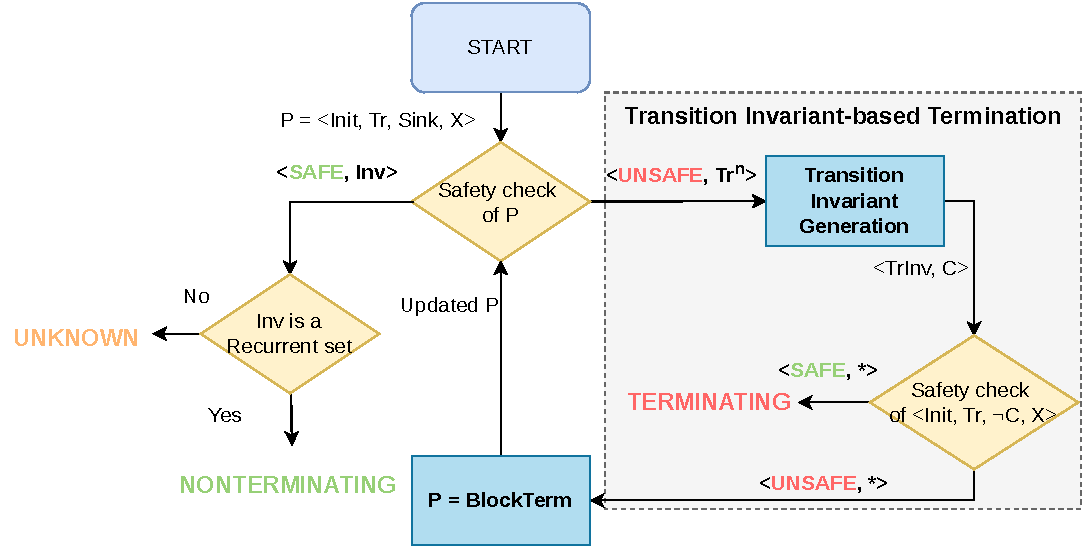
\includegraphics[width=\linewidth]{Figures/SNA+T.pdf}
    \caption{Execution Flow of Interpolation-based Transition Invariant Generation (New components are placed in a grey block, lines~\ref{SNA_Term:Synth},\ref{SNA_Term:CheckNc},\ref{SNA_Term:NEWTERM}).}
    \label{fig:SNATrInv}
\end{figure}

%  Notation is confusing, replace everything with phis, no need for phi'
%  On the second safety check use *
\begin{algorithm}[t!]
	\SetInd{0.5em}{0.5em}
    \DontPrintSemicolon
    \small
    \newcommand{\Continue}{\textbf{continue}}
    \caption{Interpolation-based Transition Invariant Generation for Proving and Disproving Termination.}
    \label{Alg:SNA_Term}
    \SetKwInOut{Input}{Input}
    \SetKwInOut{Output}{Output}
    \SetKwInOut{Data}{Data}
    \Input{Safety problem $P = \tuple{Init, Tr, Sink, X}$}
    \Output{TERM $\mid$ NONTERM $\mid$ UNKNOWN}
    \Data{$TInv$ - formula that encodes transition invariant}
    $TInv \gets \bot$ \\
    \While{$\top$} {
        \label{SNA_Term:Safety} $\tuple{res, \phi = Tr^n\ or\ Inv} \gets safetyCheck(P)$ \\
        \eIf{$res = UNSAFE$} {
            $\tuple{TInv, C} \gets \trInvSynthesis(P, Tr^n, TInv)$ \label{SNA_Term:Synth} \\
            $\tuple{res', \_} \gets safetyCheck(\tuple{Init, Tr, \lnot (C \lor Sink), X})$ \label{SNA_Term:CheckNc} \\
            \eIf{$res' = UNSAFE$} {
                $P \gets \blockTerm(P, \phi)$\label{SNA_Term:BlockTerm} \\
            }
            {
               \Return $TERM$\label{SNA_Term:NEWTERM}
            }
        }{
            \lIf{$\forall X. \phi(X) \rightarrow \exists X'. Tr(X,X') \land \phi(X')$} {
                \Return $NONTERM$ \label{SNA_Term:NONTERM}
            }
            \Return UNKNOWN
        }
        
    }
\end{algorithm}


The Algorithm~\ref{Alg:SNA_Term} takes as input a Safety Problem $P=\tuple{Init, Tr, Sink, X}$, where $Init$ and 
$Tr$ encode the initial states and transition relation, $Sink$ is the formula encoding sink states, and $X$ is 
a set of variables over which the Transition System is defined.
As an output, the algorithm returns NONTERM if TS is nonterminating, TERM if it is terminating, and UNKNOWN if the procedure 
cannot determine the final result.
The procedure maintains a formula encoding a candidate transition invariant $TInv(X,X')$ .
During the execution, $TInv$ is extended with new disjuncts, which are generated by the \trInvSynthesis procedure, and encode well-founded relations. 
Changes to the original SNA are in the lines~\ref{SNA_Term:Synth},~\ref{SNA_Term:CheckNc}, and ~\ref{SNA_Term:NEWTERM}.


Algorithm commences by analyzing the original safety problem.
Every iteration, similarly to the Algorithm~\ref{Alg:SNA}, begins with the safety check at line~\ref{SNA_Term:Safety}.
The algorithm handles two possible cases:

\paragraph{UNSAFE.} A terminating trace $Tr^n$ exists.
The algorithm calls 
\trInvSynthesis\ to extend $TInv$ and compute the coverage formula $C(X)$ (line~\ref{SNA_Term:Synth}).
\konst{Think how to include sink states to C(x), bc it does not make sense for TrInv to be valid over Sink(x).}
Then, it checks if $\lnot (C(X) \lor Sink(X))$ is reachable from the initial states (line~\ref{SNA_Term:CheckNc}).
If $\lnot (C(X) \lor Sink(X))$ is reachable, algorithm refines the safety problem by blocking 
the states deterministically leading to termination via \blockTerm, and the loop continues.
Otherwise, $TInv$ is a transition invariant over all reachable states, and algorithm concludes termination.

\paragraph{SAFE.} No sink state is reachable. 
If $\phi(X)$ is a recurrent set, the system is nonterminating. 
Otherwise, the algorithm returns UNKNOWN as the analysis is inconclusive.

\begin{example}
    Consider $TS$ from Example~\ref{Ex:Tn} with 
    $Init \triangleq x > 0$, 
    $Tr \triangleq \bigl((x'=x-1 \lor x'=x-2) \land x>0\bigr) 
    \lor \bigl(x<-10 \land x'=x-1\bigr)$, $X \triangleq \{x\}$.

    Preprocessing computes 
    $Sink \equiv x \leq 0 \land x \geq -10$.
    Then, the algorithm is called with $P=\tuple{Init, Tr, Sink, X}$.

    %

    The safety check detects a trace $Tr^1$ reaching $Sink$. 
    \trInvSynthesis produces a transition invariant candidate $TInv(X,X') \triangleq x' < x \land x' \geq 0$ and the formula $C(X) = x > 0$.
    The safety check for $\tuple{Init, Tr, \lnot (C(X) \lor Sink(X)), x}$ returns SAFE, and algorithm concludes that the transition system is terminating.
\end{example}


%-----------------------------------------------------------------------
\subsection{Correctness}
%-----------------------------------------------------------------------


This subsection proves the soundness of the introduced approach. We first prove that when algorithm returns TERM, the transition system is nonterminating,
and then we prove the correctness of the nontermination.
%  Add well-foundness definition

\begin{lemma}
    If Algorithm~\ref{Alg:SNA_Term} returns $TERM$, then the transition system $\tuple{Init, Tr, X}$ is terminating.
\end{lemma}
\begin{proof}
    $TERM$ is returned only at the line~\ref{SNA_Term:NEWTERM}, of the algorithm.
    It means that there exists a transition invariant $TInv$ which is valid over states $C(X)$, and $\lnot C(X)$ is 
    unreachable from the initial states.
    The safety problem is updated iteratively, blocking the states that deterministically lead to the termination,
    so in the end the $P = \tuple{Init', Tr', Sink, X}$, where $Init'(X) = Init(X) \land \bigwedge_{i=0}^{m} \lnot S_i(X)$
    and $Tr' = Tr(X) \land \bigwedge_{i=0}^{l} \lnot S_j(X')$ .
    According to the Lemma~\ref{Lem:Term}, Transition System $\tuple{Init', Tr', X}$ is terminating, since $TInv$ is a disjunctively well-founded
    transition invariant over all reachable states.

    Since the states satisfying $\bigvee_{i=0}^{m} S_i(X)$ and $\bigvee_{i=0}^{l} S_j(X')$ deterministically lead to the termination,
    every trace of $\tuple{Init, Tr, X}$ either follows $Tr'$ or passes through a blocked state which leads to termination.
    Hence $\tuple{Init, Tr, X}$ is terminating.
\end{proof}


\begin{lemma}
    If Algorithm~\ref{Alg:SNA_Term} returns $NONTERM$, then the transition system $\tuple{Init, Tr, X}$ is nonterminating.
\end{lemma}
\begin{proof}
    The proof of this lemma follows directly from the Lemma~\ref{Lem:NONTERM}, as the nontermination proof procedure 
    directly corresponds to one described in the Algorithm~\ref{Alg:SNA}. 
\end{proof}



\begin{example}\label{Ex:Motivation}
    Consider a transition system $TS = \tuple{Init, Tr, X}$ with 
    $X = \{x, u\}$, where $x, u$ are integer variables, $Init(X)   \triangleq u < 10 \land x > 0 $, and
    $Tr(X, X') \triangleq ((x' = x - 1 \land u' = u ) \lor (x' = x + 1 \land u' = u + 1 \land u < 10)) \land x > 0$.


    Intuitively, at each step the system either decrements $x$ (and keeps $u$ unchanged), or increments both $x$ and $u$ 
    provided $u < 10$. 
    Once $u = 10$, only the decrementing branch is available, and $x$ decreases monotonically to zero. 
    Hence $TS$ is terminating.
    The sink states are $Sink(X) \triangleq x \leq 0$.
    The initial safety problem is $P = \tuple{Init, Tr, Sink, X}$.

    \textit{Iteration 1.} $safetyCheck(P)$ returns UNSAFE with a trace $Tr^1(X^{(0)}, 
    X^{(1)})$: a sink state is reachable in one transition via the 
    decrement when $x = 1$.
    \trInvSynthesis\ constructs transition invariant:
    $TInv(X, X') \;\triangleq\; x' < x \land x > 0$. 
    The coverage formula is then computed as: $C(X) \;\triangleq\; u = 10$.
    The safety check for $\tuple{Init, Tr, \lnot C, X}$ returns UNSAFE, since states 
    with $u < 10$ are reachable from $Init$. 
    The algorithm therefore calls \blockTerm, blocking the sink-reaching 
    transition:
    $$Tr(X, X') \;\gets\; Tr(X, X') \land x' > 0 .$$

    \textit{Iteration 2.} $safetyCheck(P)$ returns SAFE with inductive invariant 
    $Inv(X) \equiv x > 0$. 
    Since $x = 1 \land u = 10$ has no  outgoing transition under the refined $Tr'$ (the decrementing 
    branch would produce $x' = 0$, which is now blocked), $Inv$ is not a recurrent set. 
    Algorithm~\ref{Alg:SNA_Term} returns \textsc{Unknown}.

    \textbf{The limitation.} The root cause why algorithm cannot prove termination is that $TInv$ does 
    not cover states with $u < 10$. 
    It captures why the system terminates when $u = 10$, but not the global argument: $u$ 
    grows until at most $u = 10$, after which $x$ decreases monotonically. 
    A complete termination proof requires a \emph{second} disjunct covering the $u < 10$ region.
    Below, we propose an extension which would allow to concentrate on the state space
    which is not covered by transition invariant.
\end{example}


\section{Extended Interpolation-based Transition Invariant Generation for Proving and Disproving Termination}
\label{Sec:Main}

Algorithm~\ref{Alg:SNA_Term} is already capable of proving termination efficiently through the construction of transition invariants.
This section describes an extension of the algorithm that aims to achieve better interaction between termination and nontermination
analysis.
Additionally, we present further extensions to the original SNA algorithm that improve overall performance. 
The high-level flow of the extended algorithm can be seen in Figure~\ref{fig:SNA++}.

\subsection{Utilising States for Which Transition Invariant is not Valid}~\label{Sec:Refinement}

Constructed transition invariant candidate can be used to guide the termination analysis.
Particularly, the Algorithm~\ref{Alg:SNA_Term} constructs the formula $C(X)$ encoding states for which the transition invariant is valid.
If $\lnot C(X)$ is reachable, it means that there exist states for which the transition invariant is not valid, and which potentially can lead to non-termination.
The intuition is to compute the reachable states $S_m$ within $\lnot C(X)$ (which corresponds to line~\ref{SNA_Refined:Sm} of Algorithm~\ref{Alg:SNA_Refined}).
Then, to attempt either prove termination or nontermination of these particular states within considered transition system (line~\ref{SNA_Refined:PushNewProblem}).


In the case of termination, the algorithm produces a witness transition invariant that extends the transition invariant of the original
system, covering previously uncovered states.
Otherwise, if nontermination is proven for $S_m$, then the original TS is also nonterminating, since $S_m$ is reachable from the initial states.


\begin{figure}[t]
    \centering
    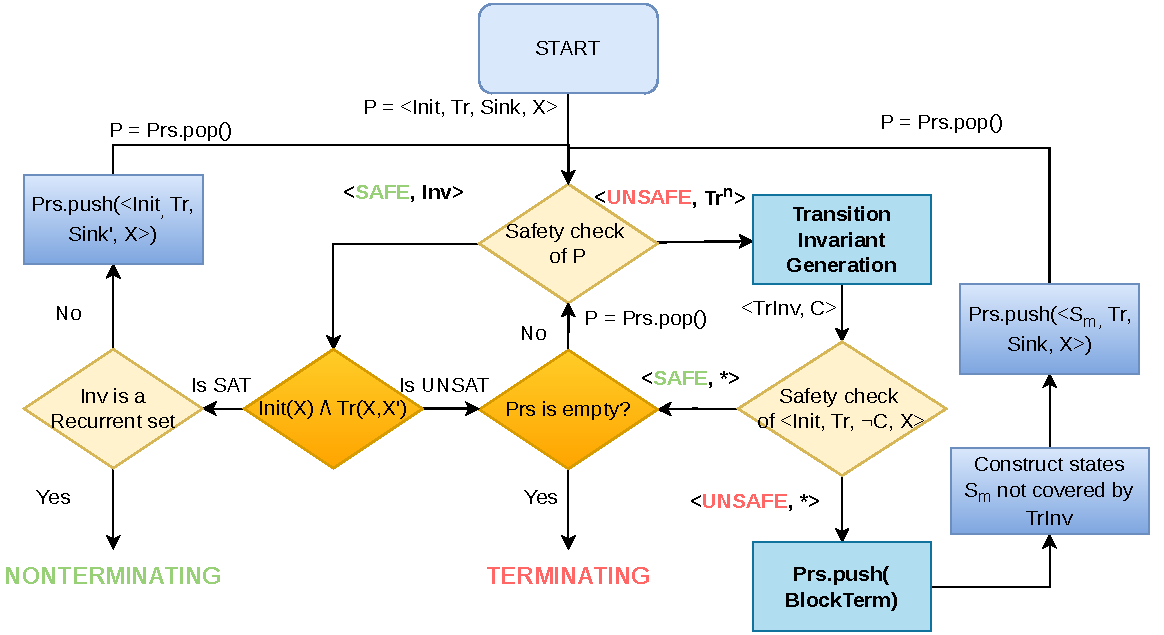
\includegraphics[width=\linewidth]{Figures/SNA++.pdf}
    \caption{Optimized Interpolation-based Termination Analysis (New components are highlighted in dark orange and dark blue colours).}
    \label{fig:SNA++}
\end{figure}

\subsection{Full Algorithm}

% Mention that A and B can be used for Algo 1
% Make people understand that C is much more important!!! Example to motivate each section!!!
% The optimized version of the algorithm is similar to the Algorithm~\ref{Alg:SNA_Term}.
% Main differences are the refinement of the safety problem, and the check for trivial termination.
% These changes allow to significantly improve the overall power and performance of the algorithm.
% In the description, we would concentrate particularly on the changes in the flow, as the rest of the algorithm is quite similar.
% Description in the line 10 - maybe explicit else - continue.

\begin{algorithm}[t!]
	\SetInd{0.5em}{0.5em}
    \DontPrintSemicolon
    \small
    \newcommand{\Continue}{\textbf{continue}}
    \caption{Extended Interpolation-based Transition Invariant Generation for Proving and Disproving Termination.}
    \label{Alg:SNA_Refined}
    \SetKwInOut{Input}{Input}
    \SetKwInOut{Output}{Output}
    \SetKwInOut{Data}{Data}
    \Input{Safety problem $P = \tuple{Init, Tr, Sink, X}$}
    \Output{TERM $\mid$ NONTERM}
    \Data{$TInv$ - formula that encodes transition invariant, $Prs$ - stack of Safety Problems to be
    analyzed for termination}
    $TInv \gets \bot$ \\
    $Prs \gets [P]$ \label{SNA_Refined:Prs} \\
    \While{$\top$} {
        \label{SNA_Refined:Extension} $\tuple{Init', Tr', Sink', X} \gets Prs.pop()$ \\
        \label{SNA_Refined:Safety} $\tuple{res, \phi = Inv\ or\ Tr^n} \gets safetyCheck(\tuple{Init', Tr', Sink', X})$ \\
        \eIf{$\tuple{res, \phi} = \tuple{UNSAFE, Tr^{n}(X^{(0)}, \dots, X^{(n)})}$} {
            $\tuple{TInv, C} \gets \trInvSynthesis(P, \phi, TInv)$ \\
            \label{SNA_Refined:CheckNc} $\tuple{res', \_} \gets safetyCheck(\tuple{Init', Tr', \lnot C, X})$ \\
            \eIf{$res' = SAFE$} {
                \eIf {$Prs = \emptyset$} {\Return $TERM$\label{SNA_Refined:NEWTERM}}
                {\Continue}
            }
            {
                $Prs.push(\blockTerm(P', \phi))$ \\
                $S_m \gets QE(\exists X^{(0)}, \dots, X^{(m-1)}, Init(X^{(0)}) \land Tr^m(X^{(0)}, \dots, X^{(m)}) \land \lnot C(X^{(m)}))$ \label{SNA_Refined:Sm}\\
                $Prs.push(\tuple{S_m, Tr', Sink', X})$\label{SNA_Refined:PushNewProblem}
            }
        }{
        %    \label{SNA_TERM:SAFE}
            \lIf{$\forall X. \phi(X) \rightarrow \exists X'. Tr'(X,X') \land \phi(X')$} {
                \Return $NONTERM$ \label{SNA_Refined:RECURRENT}
            } 
            \eIf {UNSAT ? $\phi(X) \land Tr'(X,X')$} {
                    \lIf{$Prs = \emptyset$} {\Return $TERM$ \label{SNA_Refined:TERM}}
            } {
                $Sink'(X) \gets \lnot QE(\exists X'. Tr'(X,X'))$ \label{SNA_Refined:Refinement} \\ 
                $Prs.push(\tuple{Init', Tr', Sink', X})$
            }
        }
        
    }
\end{algorithm}


Algorithm~\ref{Alg:SNA_Refined} extends Algorithm~\ref{Alg:SNA_Term} to enable more efficient termination and nontermination proving. 
\konst{Think about algo $Tr^m$ appears from nowhere.}
First, in addition to maintaining the transition invariant,
the algorithm maintains a stack of safety problems to be analyzed: $Prs$ (line~\ref{SNA_Refined:Prs}).
At each iteration, the algorithm pops a safety problem from the stack and analyzes it.
The stack allows the algorithm to focus on the termination analysis of particular reachable states within 
the TS.
The original safety problem always remains in the $Prs$ stack with blocked states that deterministically lead to termination.

The postprocessing phase of transition invariant construction is the main change to the Algorithm~\ref{Alg:SNA_Term}.
When $\lnot C$ is reachable, the extended algorithm performs two key actions: (1) it pushes the $\blockTerm$-refined problem 
(as in the original algorithm), and (2) it additionally pushes a new subproblem where  
states not covered by the transition invariant ($S_m$, line~\ref{SNA_Refined:PushNewProblem}) serve as the initial states. 
This approach allows the algorithm to concentrate on proving termination or nontermination for particular reachable states, rather than necessarily proving termination for the entire system.

Otherwise, if $\lnot C$ is not reachable, $TInv$ proves termination of the currently analyzed TS (which may be a refined TS 
previously pushed onto the stack), and the number of remaining subproblems decreases.

The following subsections describe two additional optimizations that further enhance algorithm performance:



\textit{Simple termination check.} When the safety check returns SAFE and $Inv(X)$ is not a recurrent set, 
the algorithm can additionally check whether it is possible to take a transition from the initial states by querying:
$$Init(X) \land Tr(X,X')$$
If this formula is unsatisfiable, then no transition can be taken from the initial states (or all transitions are blocked, 
meaning all reachable states deterministically lead to termination), and the system is trivially terminating. 
This check is implemented at line~\ref{SNA_Refined:TERM}.


\textit{Refinement of Recurrent sets.} When $Inv(X)$ is not a recurrent set, this is often because \blockTerm\ 
has eliminated all transitions leading to $Sink$.
This means that produced $Inv$ contains sink states itself, due to the updated $Tr$. 
New sink states can be computed as:

$$Sink'(X) = \lnot QE(\exists X'. Tr'(X,X'))$$

The formula $Sink'$ replaces $Sink$ in the safety problem, enabling the analysis to continue rather than returning UNKNOWN. 
This extension is implemented at line~\ref{SNA_Refined:Refinement}.

\begin{lemma}\label{Lem:FinalTermination}
    If Algorithm~\ref{Alg:SNA_Refined} returns $TERM$, then the original transition system $\tuple{Init, Tr, X}$ is also terminating.
\end{lemma}
\begin{proof}
    TERM is returned at line~\ref{SNA_Refined:NEWTERM} or line~\ref{SNA_Refined:TERM}.
    Similarly to Algorithm~\ref{Alg:SNA_Term}, to return $TERM$, the termination conditions need to 
    be satisfied for the transition system $\tuple{Init', Tr', X}$, where $Init'(X) = Init(X) \land \bigwedge_i \lnot S_i(X)$, 
    and $Tr'(X,X') = Tr(X,X') \land \bigwedge_j \lnot S_j(X')$.
    $\bigvee_{i=0}^m S_i(X)$ and $\bigvee_{j=0}^l S_j(X')$ are the states that deterministically lead to termination.

    \textbf{Case 1.} If $TERM$ is returned at line~\ref{SNA_Refined:NEWTERM}, then the termination proof 
    follows directly from the Lemma~\ref{Lem:Term}.

    \textbf{Case 2.} If $TERM$ is returned at line~\ref{SNA_Refined:TERM}, then the formula 
    $Init'(X) \land Tr'(X,X')$ is unsatisfiable, so no transition is reachable from $Init'$.
    This means that the transition system is terminating, since all feasible transitions in the original 
    transition system lead to deterministically terminating states.
\end{proof}

\begin{lemma}\label{Lem:FinalNontermination}
     If Algorithm~\ref{Alg:SNA_Refined} returns $NONTERM$, then the original transition system $\tuple{Init, Tr, X}$ is nonterminating.
\end{lemma}
\begin{proof}
    NONTERM is returned at line~\ref{SNA_Refined:RECURRENT}, where 
    $\phi(X)$ is a recurrent set for the current refined system  $\tuple{Init', Tr', X}$. 
    By construction, $Init'$ is reachable from  $Init$ (it is either $Init$ itself), and $Tr'(X,X') \rightarrow Tr(X,X')$.
    Based on Lemma~\ref{Lem:NONTERM}, if $NONTERM$ is returned, then there exists a recurrent set in the transition system $\tuple{Init', Tr', X}$, which 
    means that there also exists a recurrent set in the original transition system $\tuple{Init, Tr, X}$. 
    This proves nontermination.
\end{proof}

